\section{State of the Art}
Die Teilschritte einer verlustbehaftete Kompressionen können in drei Verarbeitungsarten eingeteilt werden: Transformationen, Quantisierungen und Entropie Kodierungen. Die Abbildung \ref{state:aufbau} zeigt eine vereinfachte Abfolge. Die Inputdaten werden durch ein oder mehrere Verfahren transformiert. Die Transformationen haben das Ziel die Daten aufzubereiten, sodass die folgende Quantisierungen unwichtige Informationen löschen können. Im letzten Verarbeitungsschritt werden reduzierte Information wird Entropie Kodiert. Die Entropie Kodierung versucht die Information mit einem Minimum an Daten abzubilden\\
\begin{figure}[!htbp]
	\center
	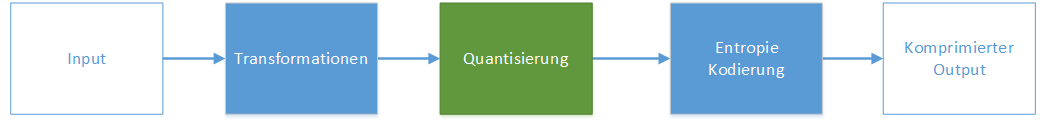
\includegraphics[width=0.8\textwidth,height=6cm,keepaspectratio]{./pictures/state/aufbau.png}
	\caption{Vereinfachter Ablauf einer verlustbehafteten Kompression}
	\label{state:aufbau}
\end{figure}

\subsection{JPEG/JFIF Bildkompression}
\begin{figure}[!htbp]
	\center
	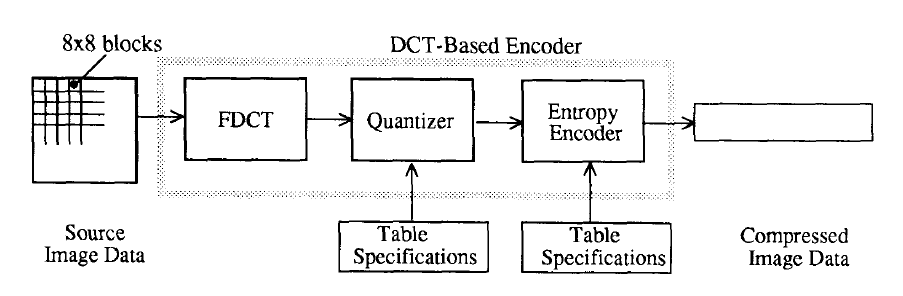
\includegraphics[width=0.8\textwidth,height=6cm,keepaspectratio]{./pictures/state/jpeg.png}
	\caption{Aufbau der JPEG Kompression \cite{wallace1992jpeg}}
	\label{state:jpeg:abb}
\end{figure}
Der JPEG/JFIF Standard\cite{wallace1992jpeg} ist eines der meist verwendeten Bildkompressionsalgorithmen für natürliche Bilder. Das Diagramm der Abbildung \ref{state:jpeg:abb} zeigt den Aufbau der Kompressionspipeline. JPEG/JFIF unterteilt das Eingabebild in $8*8$ Blöcke und führt eine Diskrete Kosinus Transformation (DCT) durch. Der Bildblock ist als Folge von Kosinus Funktionen dargestellt.\\
Die Quantisierung versucht Frequenzen, welche das menschliche Auge schlecht erkennen kann, zu quantisieren und mit weniger Präzision darzustellen. Wenn die Quantisierung gut gewählt wurde, kann das menschliche Auge das dekomprimierte Bild nicht vom Original unterscheiden. JPEG/JFIF bietet vorgefertigte Quantisierungstabellen an. Der Benutzer kann aber auf den anwendungsfall spezialisierte Tabellen anwenden. Wie die Quantisierungstabelle optimal gewählt wird, ist ein aktives Forschungsfeld \cite{wu1993rate:jpeg} \cite{wang2001designing:jpeg} und kann von Anwendungsfall zu Anwendungsfall unterschiedlich sein.\\
Nach der Quantisierung werden die quantisierten Blöcke im Zick-Zack-Muster\cite{wallace1992jpeg} angeordnet. So soll die Entropie Kodierung ähnliche Muster findent und eine höhere Kompressionsrate ereichen. JPEG/JFIF führt eine Run-Length\cite{wiki:rle} und eine Huffman-Kodierung\cite{huffman1952method} durch.

Wenn für die Kompression von wissenschaftlichen Daten eine Diskrete Kosinus Transformation eingesetzt wird, kann ein ähnlicher Aufbau verwendet werden wie der JPEG/JFIF Standard. Für eine optimale Kompression wird die Umsetzung der einzelnen Schritte vom Standard abweichen.

\subsection{Point Cloud Kompression} \label{state:pointcloud}
\begin{figure}[!htbp]
	\center
	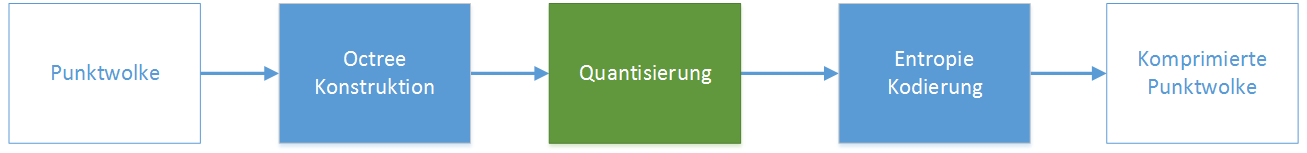
\includegraphics[width=0.8\textwidth,height=6cm,keepaspectratio]{./pictures/state/pointcloud.png}
	\caption{Aufbau einer Octree basierten Point Cloud Kompression.}
	\label{state:pointcloud:abb}
\end{figure}
3d Laser Sampling Geräte produzieren grosse Mengen an dreidimensionalen Punkten von alltäglichen Objekten. Die Kompression von solchen Punktwolken ist ein aktives Forschungsfeld. Eine vorgeschlagene Kompression  von Schnabel und Klein \cite{schnabel2006octree} verwendet Octrees \cite{wiki:octree}. Das Diagramm der Abbildung \ref{state:pointcloud:abb} verdeutlicht den Ablauf.\\
Die dreidimensionalen Punkte werden in einem Octree mit einer begrenzten Anzahl an Levels abgelegt. Im Quantisierungsschritt werden die Punkte durch die Zellenmittelpunkte des Octrees ersetzt. Die Anzahl an Levels ist gleichzusetzen mit der Genauigkeit in Bits welche für jede Koordinatenachse zur Verfügung stehen. Wenn die Levels auf $8$ begrenzt sind, steht für jede Achse $8$ Bit Genauigkeit zur Verfügung.\\
In der Entropie Kodierung wird der Octree in Breadth-First Ordnung binär abgebildet ($0$ für leere Knoten, $1$ für befüllte Knoten). Jeder Level im Octree repräsentiert eine Approximation der Punktwolke. Durch  die Breath-First Ordnung werden die ungenaueren Approximationen zuerst abgelegt. Diese Eigenschaft wird mit einer Prädiktiven Kodierung ausgenutzt: Aus den vorhergehenden Levels wird die Punktverteilung des nächsten Level vorhergesagt. Es wird nur Abweichung der Vorhersage gespeichert. Kann der Prädiktor eine zuverlässige Vorhersage treffen, wird eine hohe Kompressionsrate erreicht.

Um die Point Cloud Kompression auf die Feldlinien anzuwenden muss die Information gespeichert werden, welcher Punkt zu welcher Linie gehört. Schnabel und Klein stellen einen angepassten Algorithmus vor, welcher eine Punktwolke mit Farbinformationen komprimiert. Die Farbinformation kann verwendet werden um einen Punkt einer Feldlinie zuzuordnen. Weiter muss die Prädiktive Kodierung angepasst werden: Schnabel und Klein nehmen an, dass die Punktwolke eine Oberfläche darstellen. Die Feldlinien bilden im Allgemeinen keine Oberfläche und benötigen deshalb eine andere Prädiktive Kodierung.

\subsection{Curve Fitting}
Curve Fitting ist ein Prozess, welcher ein Signal durch eine oder mehrere Funktionen abbildet. Es ist zwischen einem exakten Curve Fitting und einer Approximation zu unterscheiden. Die exakte Repräsentation wird für die Signalinterpolation und eine Approximation in der Rauschunterdrückung verwendet. Eine Datenkompression ist mit Curve Fitting möglich, wenn die Parameter der approximierenden Funktionen weniger Speicherplatz benötigen, als das Signal.\\
Unser et al \cite{unser1993b:spline} zeigt ein Algorithmus, welcher ein diskretes Signal als Folge von B-Splines darstellt. Die Anwendungsmöglichkeiten des Verfahrens sind nicht auf Interpolation und Rauschunterdrückung beschränkt: Unser et al. stellt im Ansatz eine Bildkompression vor mittels B-Splines \cite{unser1993b2:spline}. Der Vorteil des Verfahrens ist, dass sich die Artefakte der Kompression als Rauschunterdrückung und Schärfung des Originalbildes ausdrücken.

Eine Datenkompression mit Curve Fitting ist im Vergleich mit der Kosinus Transformation weniger erforscht. Es sind ebenfalls keine Kompressionsstandards bekannt, welche ein Curve Fitting für die Datenkompression verwenden. Ein Kompressionsverfahren zu entwickeln zieht zusätzlichen Aufwand mit sich als Verfahren, welche in der Datenkompression etabliert sind.

\subsection{Compressive Sensing}
Compressive Sensing ist ein Verfahren, welches ein Signal mit einer minimalen Anzahl an vordefinierten Funktionen darstellt (sparse representation). Die Funktionen sind durch keine Rahmenbedingungen begrenzt, jede allgemeine Funktion kann im Compressive Sensing verwendet werden. 

Das Überführen in die sparse representation ist ein $np-hard$ Problem \cite{wiki:npHard}. Es existieren Heurisiken wie Orthogonal Matching Pursuit\cite{tropp2007signal}, welches Approximation der sparse representation mit linearer Komplexität erstellt. Die Approximation ist für praktische Anwendungsfälle wie eine Datenkompression mittels Compressive Sensing ausreichend genau.

Mit einem allgemeinen Dictionary von vordefinierten Funktionen ist jedes Signal rekonstruierbar. Die Stärke des Compressive Sensing Ansatzes ist, dass das Dictionary auf die Signale optimiert werden kann. Der K-SVD \cite{bryt2008compression} Algorithmus erlernt mittels Unsupervised Learning ein Dictionary, welches auf die zu kodierenden Signale zugeschnitten ist. 

Compressive Sensing hat das Potential eine hohe Kompressionsrate zu erreichen. Die Feldlinien sind oft ähnlich und unterscheiden sich hauptsächlich in Rotation, Verschiebung und Skalierung. Mit einem auf Feldlinien angepasstes Dictionary kann eine Feldlinie durch wenige Funktionen approximiert werden.

\subsection{Entropie Kodierung}
Die Entropie Kodierung findet in allen Bereichen der Informatik Anwendungen. Ziel der Kodierung ist die gleiche Information mit einem Minimum an Daten darzustellen. Verlustbehaftete Kompressionsverfahren reduzieren die Information und verwenden im letzten Schritt eine Entropie Kodierung um die Datenmenge zu reduzieren.

Es ist zwischen spezialisierten und allgemeinen Entropie Kodierer zu unterscheiden. Unter den spezialisierten Verfahren ist Beispielswiese die Arbeit von Ratanaworabhan et al.\cite{ratanaworabhan2006fast} einzuordnen, welche in der Lage ist Floating Point Daten performant zu kodieren und dekodieren.
 
Unter den allgemeinen Verfahren sind Archivierer wie GZIP\cite{website:gzip}, 7-ZIP\cite{website:7zip} und RAR\cite{website:rar} angesiedelt. Archivierungsverfahren finden in allen Bereichen Anwendung und dienen in der Entwicklung von spezialisierten Kodierer als Messbasis. Im Vorfeld wurde die Kompressionsraten von GZIP, 7-ZIP und RAR von Feldliniendaten verglichen, wobei RAR die höchsten Raten erreichen konnte.\\
Die Verfahren der Archivierer bestehen aus Kombinationen von Entropie Kodierungen. Zum Beispiel verwendet GZIP den DEFLATE Algorithmus\cite{deutsch1996deflate}, welcher aus einer Kombination von LZ77\cite{ziv1977universal} und Huffman\cite{huffman1952method} Kodierung besteht. Rar hingegen besitzt unterschiedliche Kombinationen und wählt das Verfahren aus, welches die Inputdaten optimal kodieren kann. Dadurch kann RAR für unterschiedlichen Anwendungsfällen eine hohe Kompressionsrate erreichen. Die RAR Kompression ist urheberrechtlich Geschützt und die verwendeten Algorithmen sind nicht bekannt.